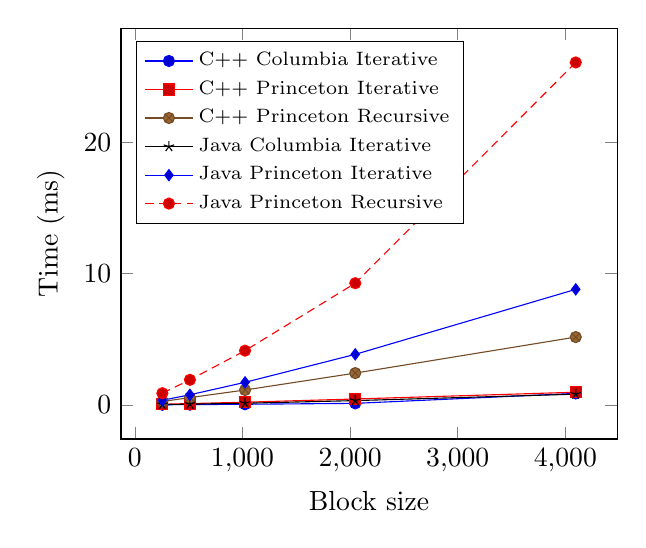
\begin{tikzpicture}
\begin{axis}[xlabel={Block size},ylabel={Time (ms)},width=0.65\linewidth,legend pos=north west,scaled y ticks = false,legend cell align=left,legend style={font=\scriptsize}]
\addplot coordinates {
(256, 0.0160)
(512, 0.0223)
(1024, 0.0516)
(2048, 0.1206)
(4096, 0.8794)
};
\addplot coordinates {
(256, 0.0541)
(512, 0.1038)
(1024, 0.2082)
(2048, 0.4536)
(4096, 0.9690)
};
\addplot coordinates {
(256, 0.2642)
(512, 0.5573)
(1024, 1.1380)
(2048, 2.4265)
(4096, 5.1699)
};
\addplot coordinates {
(256, 0.0290)
(512, 0.0603)
(1024, 0.1289)
(2048, 0.3302)
(4096, 0.8200)
};
\addplot coordinates {
(256, 0.3547)
(512, 0.7740)
(1024, 1.7228)
(2048, 3.8546)
(4096, 8.8053)
};
\addplot coordinates {
(256, 0.8938)
(512, 1.9155)
(1024, 4.1350)
(2048, 9.2740)
(4096, 26.0912)
};
\legend{C++ Columbia Iterative,C++ Princeton Iterative,C++ Princeton Recursive,Java Columbia Iterative,Java Princeton Iterative,Java Princeton Recursive}
\end{axis}
\end{tikzpicture}
